\section{Durchführung}
\begin{frame}
  \frametitle{Versuchsaufbau- und durchführung}
\begin{figure}
  \centering
  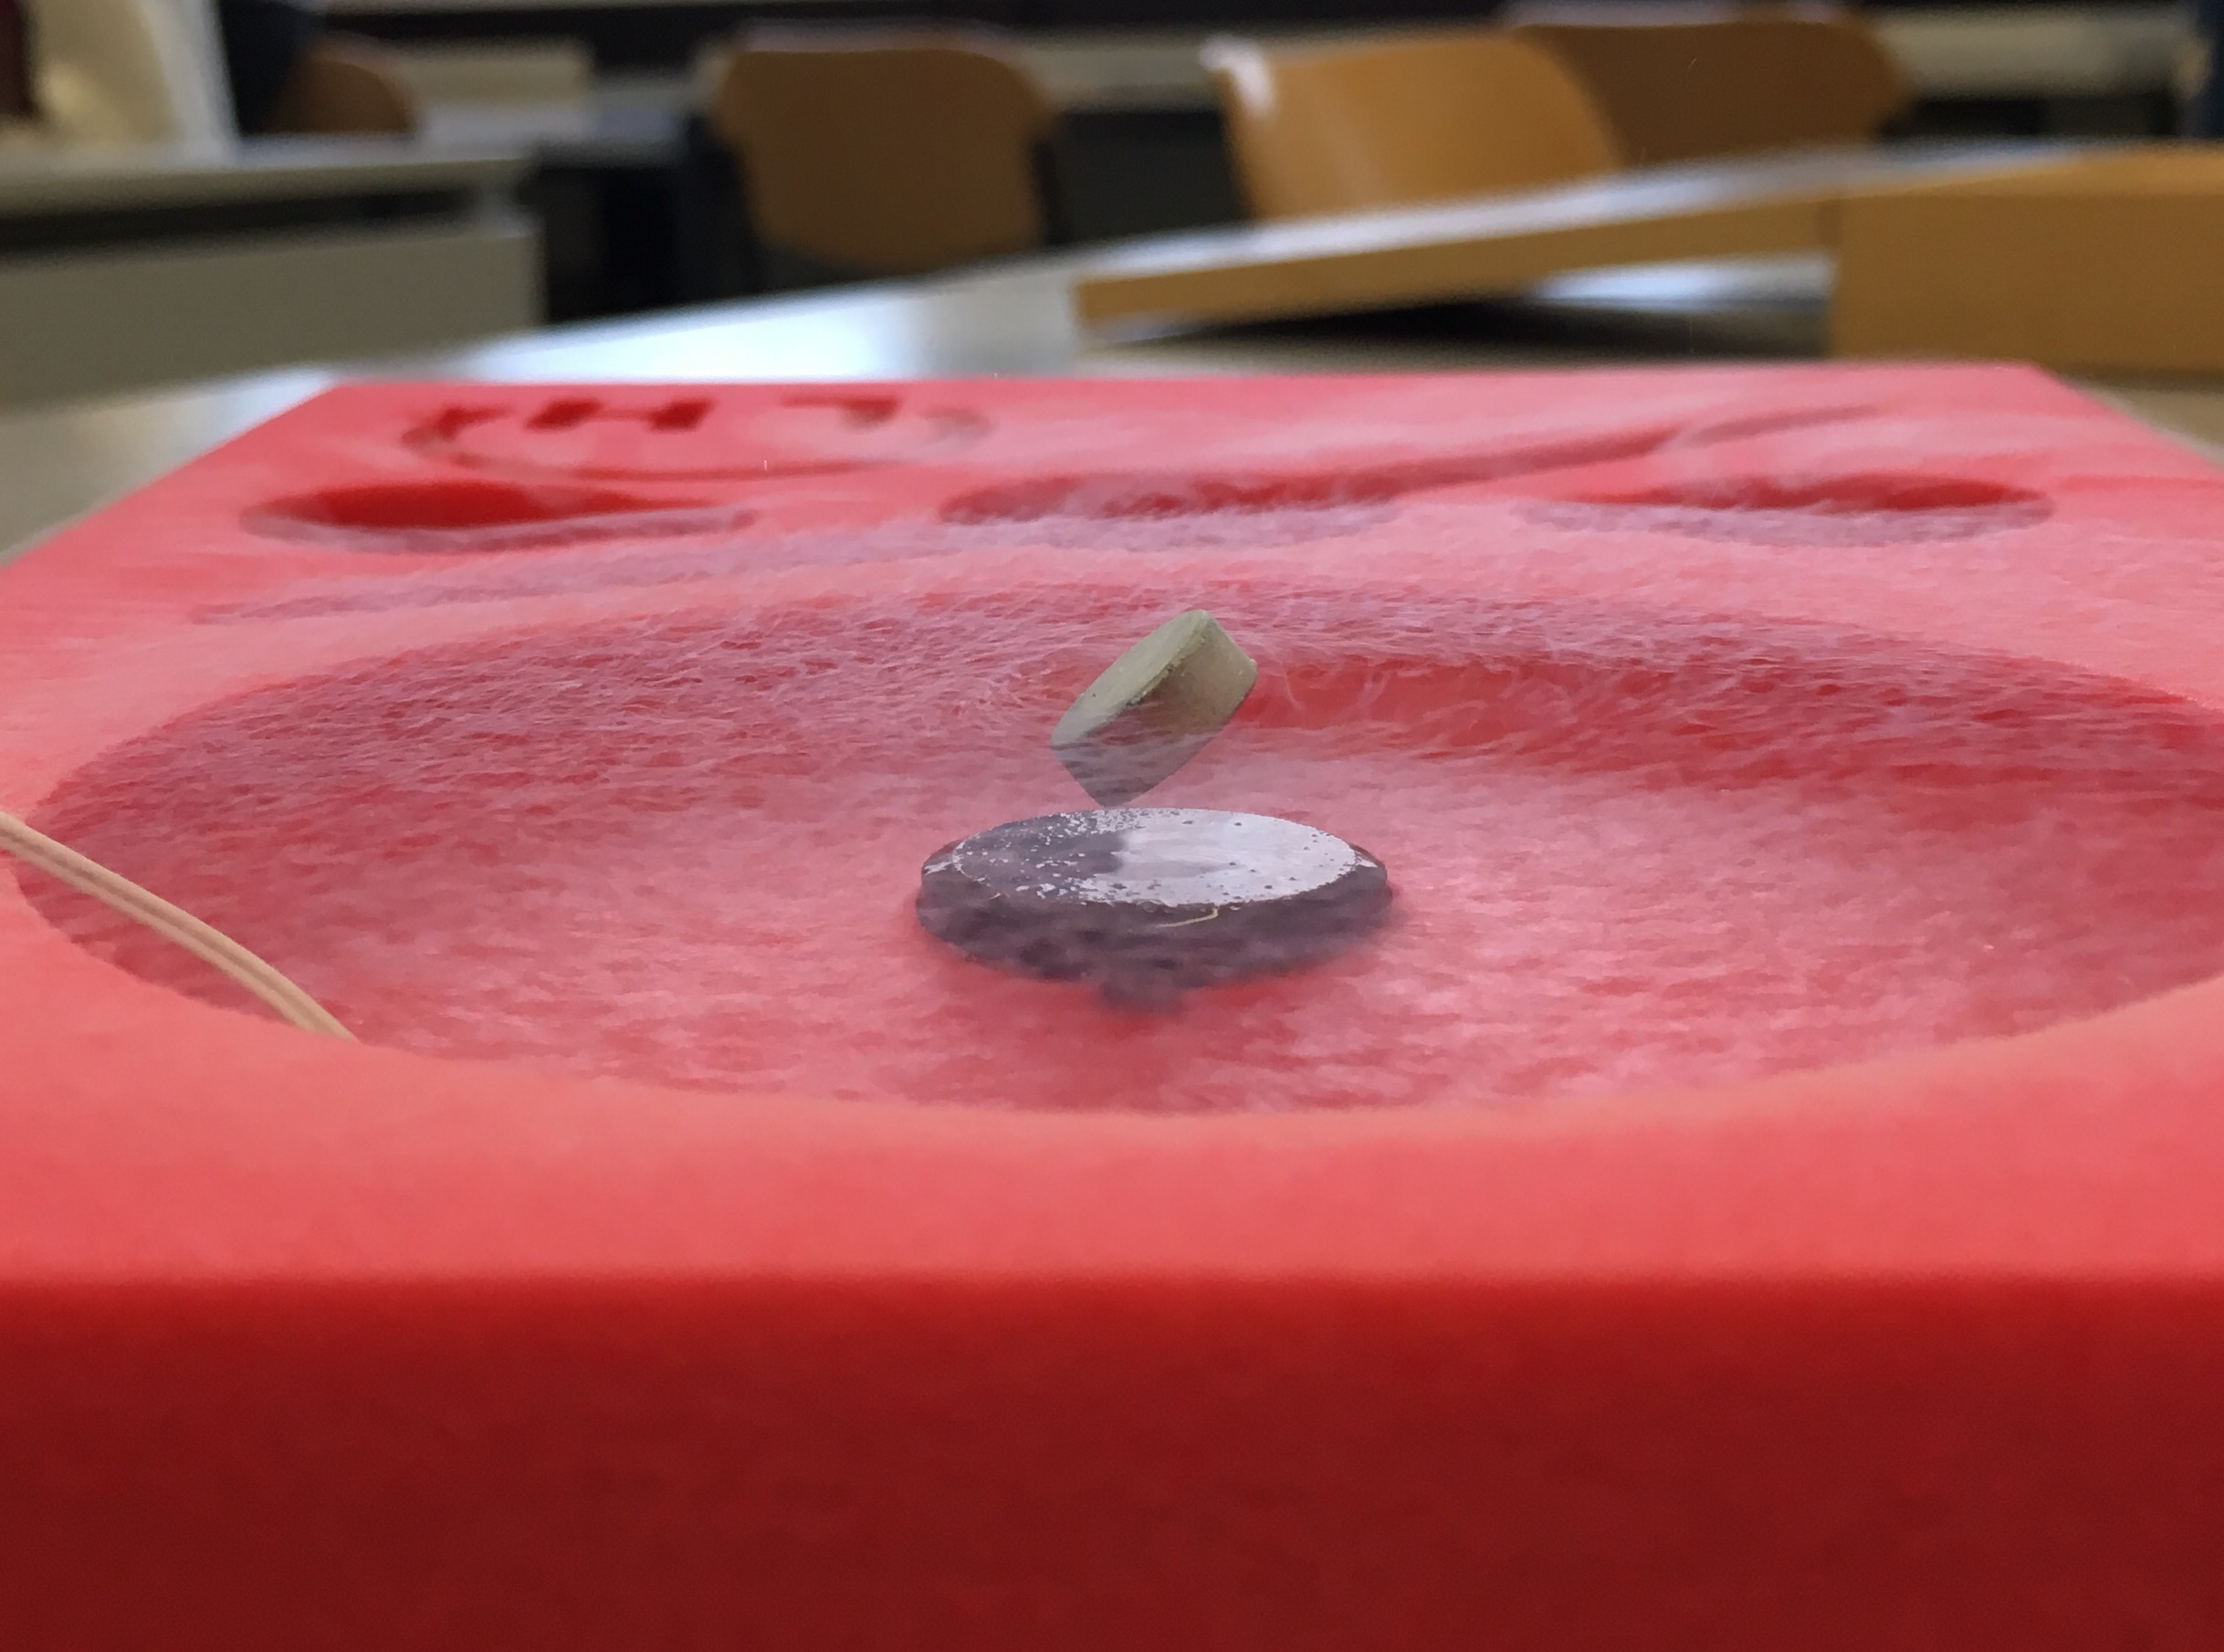
\includegraphics[width=0.7\textwidth]{bilder/versuchsaufbau.jpg}
\caption{Foto des Versuchsaufbau und des Meißner-Ochsenfeld-Effektes }
  \label{fig: versuchsaufbau}
\end{figure}
\end{frame}
\begin{frame}
  \frametitle{Versuchsaufbau- und durchführung}
\begin{figure}
  \centering
  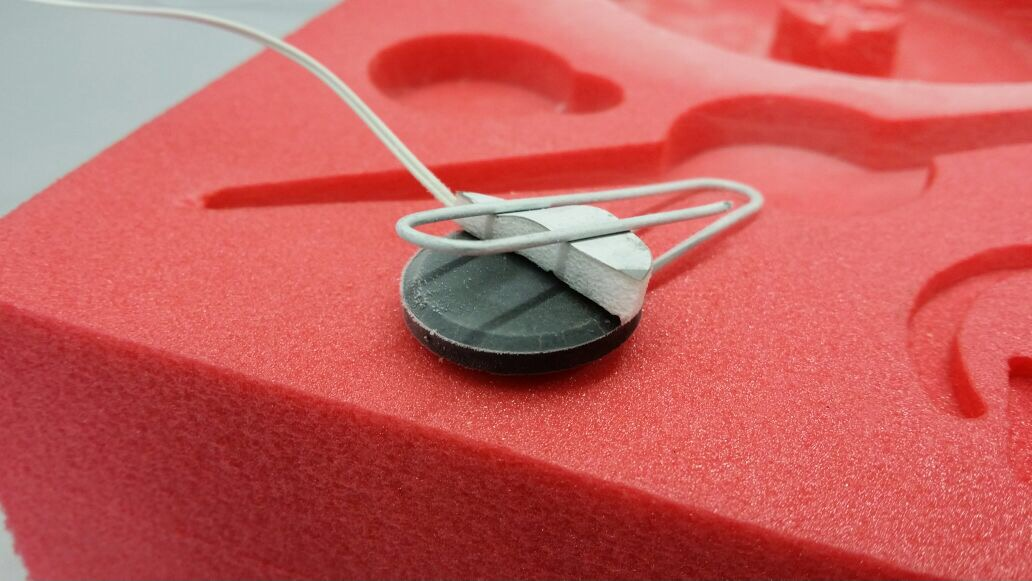
\includegraphics[width=0.7\textwidth]{bilder/versuchsaufbau_2.JPG}
\caption{Befestigung des Thermoelements am Supraleiter}
  \label{fig: versuchsaufbau_2}
\end{figure}
\end{frame}
\begin{frame}{Temperaturmessung}
    \begin{itemize}
      \item{Thermoelement}
      \item{Zur Kalibierung wurden Eiswasser und flüssiger Stickstoff verwendet}
      \item{Als Referenztemperatur diente Eiswasser}
    \end{itemize}
\end{frame}
\begin{frame}
  \frametitle{Auswertung der kritischen Temperatur}
\begin{columns}
  \begin{column}{0.52\textwidth}
\begin{table}
  \centering
  \caption{Gemessene kritische Temperaturen}
  \label{tab:messwerte}
  \begin{tabular}{SSS}
  \toprule
  {Messwert} & {Spannung in $\si{\milli\volt}$}  &  {Temperatur in $\si{\celsius}$}  \\
  \midrule
   1  & -5.70  & -192.68\\
  2  & -5.77  & -195.00\\
  3  & -5.77  & -195.00\\
  4  & -5.76  & -194.67\\
  5  & -5.76  & -194.67\\
  6  & -5.75 & -194.34\\
  7  & -5.76 & -194.67\\
  8  & -5.76  & -194.67\\
  9  & -5.75  & -194.34\\

  \bottomrule
  \end{tabular}
\end{table}

\end{column}
\pause
\begin{column}{0.52\textwidth}
\begin{align*}
  \qquad T_{\mathrm{mittel}}&=-194.45 \pm 0.66 \,\si{\celsius}\\
  \hfill \\
  \quad T_{\mathrm{theo}}&=-180\,\si{\celsius}  \\
  \hfill \\
  \quad \Delta T&= 14.45\pm 0.66\,\si{\celsius} \quad (-7\%)
\end{align*}
\end{column}
\end{columns}

\end{frame}
